% Pablo Baeyens (@pbaeyens)
% Email: pbaeyens31+github@gmail.com
% Licencia: CC BY-SA 3.0

%% Paquetes y configuración %

% Beamer
\PassOptionsToPackage{unicode}{hyperref}  % Evita errores con caracteres no ASCII
\PassOptionsToPackage{naturalnames}{hyperref} % tex.stackexchange.com/questions/10555
\documentclass[compress]{beamer}

% Idioma
\usepackage[spanish]{babel} % Traducciones
\usepackage[utf8]{inputenc} % Uso de caracteres UTF-8
\usepackage{lmodern}        % Fuentes de tamaño arbitrario
\usepackage[T1]{fontenc}    % Permite copiar y evita errores
\uselanguage{Spanish}       % Traducciones beamer
\languagepath{Spanish}      % (tex.stackexchange.com/questions/168208)

% Matemáticas
\usepackage{amsfonts}
\usepackage{amsmath}
\usepackage{amssymb}

% Colores
\definecolor{backg}{HTML}{F2F2F2}    % Fondo
\definecolor{title}{HTML}{bdc3d1}    % Títulos
\definecolor{comments}{HTML}{BDBDBD} % Comentarios
\definecolor{keywords}{HTML}{08388c} % Palabras clave
\definecolor{strings}{HTML}{FA5858}  % Strings
\definecolor{links}{HTML}{2C2C95}    % Enlaces
\definecolor{bars}{HTML}{045FB4}     % Barras (gráfico)

% Código
\usepackage{listings}
\lstset{
language=[LaTeX]TeX,
basicstyle=\footnotesize,
morekeywords={href,uselanguage,languagepath,column},
otherkeywords={pause,usetheme,usecolortheme,useinnertheme,titlepage,tableofcontents,subtitle},
breaklines=true,
backgroundcolor=\color{backg},
keywordstyle=\color{keywords},
commentstyle=\color{comments},
stringstyle=\color{strings},
tabsize=2,
% Acentos, ñ, ¿, ¡ (tex.stackexchange.com/questions/24528)
extendedchars=true,
literate={á}{{\'a}}1 {é}{{\'e}}1 {í}{{\'i}}1 {ó}{{\'o}}1
         {ú}{{\'u}}1 {ñ}{{\~n}}1 {¡}{{\textexclamdown}}1
         {¿}{{?`}}1
}

% Gráficos
\usepackage{pgfplots}
\pgfplotsset{width=7cm,compat=1.8} % Opciones para gráficos

% Emoticonos
\usepackage{wasysym}

% tikz
\usepackage{tikz}
\usetikzlibrary{mindmap,trees,shadows}
\tikzset{ % Genera overlays
    invisible/.style={opacity=0},
    visible on/.style={alt={#1{}{invisible}}},
    alt/.code args={<#1>#2#3}{\alt<#1>{\pgfkeysalso{#2}}{\pgfkeysalso{#3}}},
}

%% Comandos %%
\newcommand{\ejemplo}[1]{\lstinputlisting{./examples/#1}} % Mostrar código de ejemplos
\newcommand{\muestra}[1]{\input{./examples/#1}}           % Mostrar ejemplos
\newcommand{\seccion}[1]{\input{./sections/#1}}           % Incluir secciones
\newcommand{\espacio}{\vspace*{\baselineskip}}            % Añade espacios
\newcommand{\beamer}{\texttt{beamer} }                    % Estilo único para beamer
\newcommand{\enlace}[3]{\href{#1}{\textbf{#2}} - {\small #3}}  % Estílo único para refs
\newcommand{\comando}[1]{{\color{black}\textbackslash}{\color{keywords}#1}}

%% Temas %%
% Tema y tema de color
  \usetheme{Szeged}
  \usecolortheme{crane}
% \useinnertheme{circles}
  \setbeamercovered{transparent}
% Colores bloques
%  \setbeamercolor{block title}{bg=title,fg=links}
%  \setbeamercolor{block body}{bg=backg,fg=black}
%  \setbeamercolor{block title alerted}{fg=red!70!black,bg=title!92!red}
%  \setbeamercolor{block body alerted}{fg=black,bg=backg}
%  \setbeamercolor{block title example}{fg=green!70!black,bg=title!92!green}
%  \setbeamercolor{block body example}{fg=black,bg=backg}
% Enlaces (tex.stackexchange.com/questions/13423)
\hypersetup{colorlinks,linkcolor=,urlcolor=links}
% Quita enlaces de navegación (stackoverflow.com/questions/3017030)
\setbeamertemplate{navigation symbols}{}
% Quita barra inferior (stackoverflow.com/questions/1435837)
\setbeamertemplate{footline}{}
% Evita warnings boxes
\hfuzz=20pt
\vfuzz=20pt
% Evita wranings itemize
\renewcommand\textbullet{\ensuremath{\bullet}}

% tikz
\usepackage{tikz}
\usetikzlibrary{shapes.multipart}

%% Título y otros %%
\title{Presentación práctica de eficiencia}                                               % Título
\subtitle{Asignatura: Algorítmica}                                  % Subtítulo
\author{Rubén Morales Pérez
		\and Francisco Javier Morales Piqueras
		\and Bruno Santindrian Manzanedo
		\and Ignacio de Loyola Barragan Lozano
		\and Francisco Leopoldo Gallego Salido}
\date{\today}                                                            % Fecha


%%%%%%%%%%%%%%%%%%%%%%%%%%%%%%%%%%%%%%%%%%%%%%%%%%%%%%%%%%%%%%%%

%% Presentación %%
\begin{document}

\begin{frame}
\titlepage
\end{frame}
\begin{frame}{Índice}
  \hypertarget{index}{}
  \tableofcontents
\end{frame}


\section{Presentación}
\subsection{Introducción}
\begin{frame}
	\begin{block}{Eficiencia}
	Hemos usado los siguientes algoritmos en esta práctica
	\end{block}
	
\begin{columns}  
\begin{column}{5cm}   
	\vspace*{1cm}
	\begin{block}{Ordenaci\'on} 
	\begin{itemize}
		\item Burbuja
		\item Inserción
		\item Selección
		\item Mergesort
		\item Quicksort
		\item Heapsort
	\end{itemize}      
	\end{block}            
\end{column}	

\begin{column}{5cm} 
	\begin{block}{Otros}
	\begin{itemize}
		\item Fibonacci
		\item Hanoi
		\item Floyd
	\end{itemize}    
	\end{block}	                 
\end{column}  
\end{columns}	
\end{frame}

%%%%%%%%%%%%%%%%%%%%%%%%%%%%%%%%%%%%%%%%%%%%%%
\begin{frame}
	\begin{block}{Script}
		El siguiente script automatizaba el proceso de obtención de las gráficas y los 				datos.		
	\end{block}
	
	\begin{exampleblock}{script.sh}
		g++ -std=c++11 ../src/algoritmo.cpp
		
		nelementos=200
				
		while [ 	\$nelementos -lt 10000 ]; do
		
    		\hspace{0.75cm}	./a.out \$nelementos >> datos.dat
    			
    		\hspace{0.75cm}	let nelementos=nelementos+100
    			
		done
		

		gnuplot ./gnuplot/algoritmo.gp \# Salida: fichero.jpeg
		
		mv fichero.jpeg ../Graficas/Algoritmo/algoritmo.jpeg
		
		mv datos.dat ../Graficas/Algoritmo/Datos/algoritmo.dat
	\end{exampleblock}
	
\end{frame}
%%%%%%%%%%%%%%%%%%%%%%%%%%%%%%%%%%%%%%%%%

\begin{frame}
	\begin{block}{Scripts de gnuplot}
		Podemos hacer que gnuplot automatice su trabajo.
		
		Suponemos que el fichero donde están los datos es "datos.dat", como indicamos anteriormente los scripts de gnuplot se ejecutan:
		
		\hspace{2cm} gnuplot algoritmo.gp
	\end{block}
	\pause
	
	\begin{columns}
	\begin{column}{5cm}
	\begin{exampleblock}{algoritmo.gp}
	set terminal pngcairo
	
	set output "fichero.jpeg"
	
	set title ''Eficiencia algoritmo"
	
	set xlabel "Tamaño del vector"

	set ylabel "Tiempo (s)"

	set fit quiet

	f(x) = a*x*x+b*x+c

	fit f(x) "datos.dat" via a, b, c

	plot "datos.dat", f(x)
	\end{exampleblock}
	\end{column}
	\pause
	
	\begin{column}{5cm}
	\begin{block}{Funciones ajustadas}
		\[f(x)=ax^3 + bx^2 + cx + d\]
		\[g(x)=ax^2 + bx + c\]
		\[h(x)=ax\cdot log_2(x)\]
		\[i(x)=a \cdot ((1+ \sqrt(5))/2)^x\]
	\end{block}
	\end{column}
	
	\end{columns}
\end{frame}

%%%%%%%%%%%%%%%%%%%%%%%%%%%%%%%%%%%%%%%
\begin{frame}
	\begin{alertblock}{Ordenador usado para la ejecuci\'on}
	HP Pavilion g series (Pavilion g6)

	Sistema operativo: ubuntu 14.04 LTS

	Memoria: 3.8 GiB (4Gb)

	Procesador: Inter Core i3-2330M CPU @ 2.20GHz x 4

	Gráficos: Intel Sandybridge Mobile

	Tipo de SO: 64 bits

	Disco: 487.9 GB	
	\end{alertblock}
\end{frame}


%%%%%%%%%%%%%%%%%%%%%%%%%%%%%%%%%%%%%%
\section{Algoritmos de ordenación}
\subsection{Burbuja}
\begin{frame}{Burbuja}
	\begin{block}{Función}
	Este algoritmo tiene una eficiencia cuadrática, debemos ajustar una función del tipo
	$f(x)= ax^2 + bx +c$
	\end{block}
	\pause

	\begin{block}{Ajuste}
	$f(x) = a\cdot x^2 + b\cdot x + c$
	
	En el ajuste también tenemos un margen de error:
	
	$\left\{ \begin{array}{c}
	a               = 4.31433\cdot 10^{-9}      \pm 2.378\cdot 10^{-10}    (5.511\%) \\
	b               = 3.94506\cdot 10^{-6}      \pm 2.476\cdot 10^{-6}    (62.75\%) \\
	c               = -0.00311235     \pm 0.005425     (174.3\%)
	\end{array}\right.$
	\end{block}
\end{frame}

\begin{frame}	
	\begin{alertblock}{Imagen}
	\begin{center}
	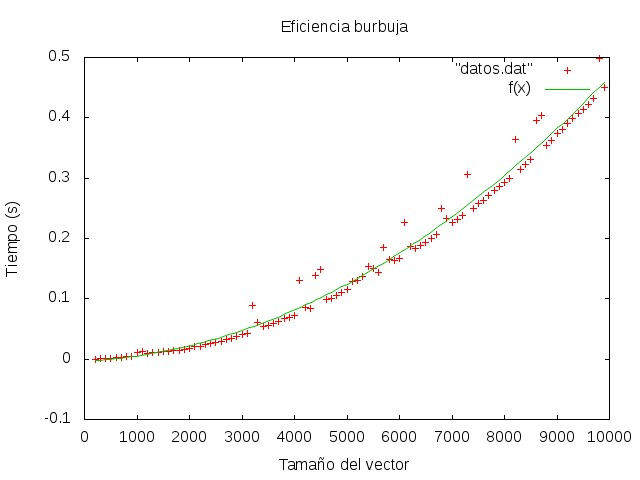
\includegraphics[scale=0.55]{../Graficas/Burbuja/burbujaO0_ruben.jpeg}
	\end{center}
	\end{alertblock}
\end{frame}


%%%%%%%%%%%%%%%%%%%%%%%%%%%%%%%%%%%%%%%%%%%%%%%%%%%%%%
\subsection{Inserción}
\begin{frame}{Inserción}
	\begin{block}{Función}
	Aunque el algoritmo de inserción tenga una eficiencia $O(n^2)$ tiene una constante 			multiplicativa menor que el burbuja, y similar al selección.
	\end{block}
	
	\begin{block}{Ajuste}
	$f(x) = a\cdot x^2 + b\cdot x + c$
	
	$\left\{ \begin{array}{c}
	a               = 2.36229\cdot 10^{-9}      \pm 2.503\cdot 10^{-10}    (10.6\%) \\
	b               = -2.27723\cdot 10^{-6}     \pm 2.606\cdot 10^{-6}    (114.5\%) \\
	c               = 0.00096037       \pm 0.005712     (594.8\%)
	\end{array}\right.$	
	\end{block}
\end{frame}

\begin{frame}
	\begin{alertblock}{Imagen}
	\begin{center}
	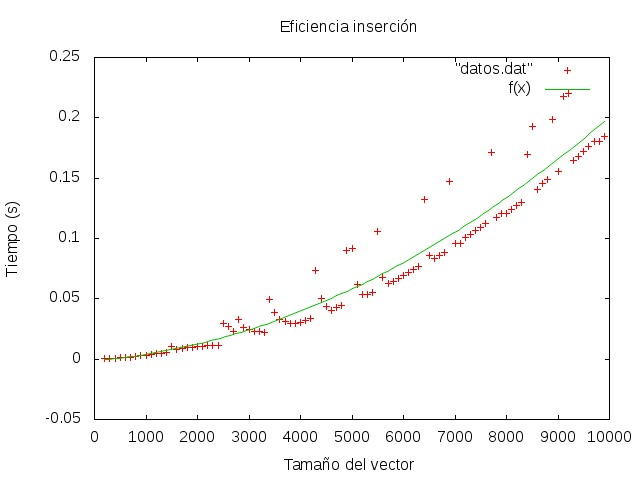
\includegraphics[scale=0.55]{../Graficas/Insercion/insercionO0_ruben.jpeg}
	\end{center}
	\end{alertblock}
\end{frame}


%%%%%%%%%%%%%%%%%%%%%%%%%%%%%%%%%%%%%%%%%%%%%%%%%%
\subsection{Selección}
\begin{frame}{Selección}
	\begin{block}{Función}
		Este algoritmo tiene dos partes una ordenada y otra no, en cada iteración coge el 			máximo/mínimo de los elementos no ordenados y los inserta en los ordenados.
	\end{block}
	
	\begin{block}{Ajuste}
	$f(x) = a\cdot x^2 + b\cdot x + c$
	
	$ a               = 2.36327\cdot 10^{-9}      \pm 3.232\cdot 10^{-11}    (1.368\%) $
	\end{block}
\end{frame}

\begin{frame}
	\begin{alertblock}{Imagen}
	\begin{center}
	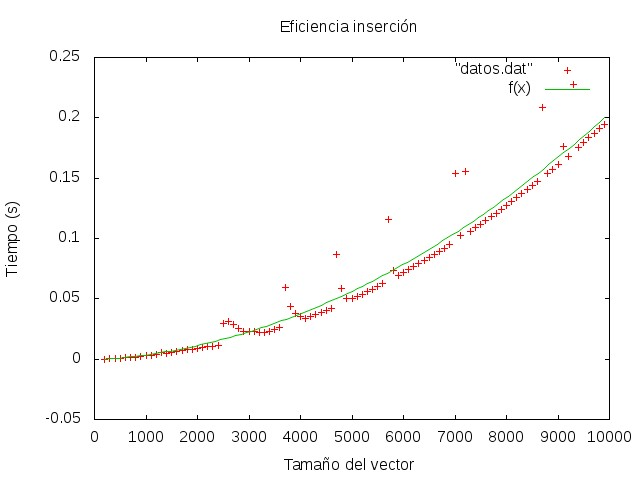
\includegraphics[scale=0.55]{../Graficas/Seleccion/seleccionO0_ruben.jpeg}					\end{center}
	\end{alertblock}
\end{frame}



%%%%%%%%%%%%%%%%%%%%%%%%%%%%%%%%%%%%%%%%%%%%%%%%%%%
\subsection{Mergesort}
\begin{frame}{Mergesort}
	\begin{block}{Función}
	Siguiente algoritmo de ordenación: mergesort
	\end{block}
	
	\begin{block}{Ajuste}
	$ f(x) = a\cdot x\cdot log_2(x)$
	
	$ a               = 3.5231\cdot 10^{-8}       \pm 1.191\cdot 10^{-9}    (3.382\%) $
	\end{block}
\end{frame}
\begin{frame}
	\begin{alertblock}{Imagen}
	\begin{center}
	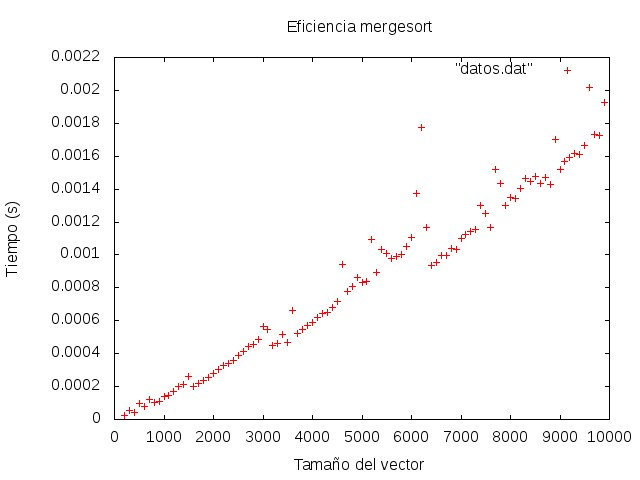
\includegraphics[scale=0.55]{../Graficas/Mergesort/mergesortO0_bruno.jpeg}
	\end{center}
	\end{alertblock}
\end{frame}

%%%%%%%%%%%%%%%%%%%%%%%%%%%%%%%%%%%%%%%%%%%%%%%%%%%%

\subsection{Quicksort}
\begin{frame}{Quicksort}
	\begin{block}{Función}
	El algoritmo de ordenación más rápido en término medio: quicksort
	\end{block}
	
	\begin{block}{Ajuste}
	$f(x) = a\cdot x\cdot log_2(x)$

	$a               = 2.3704\cdot 10^{-8}       \pm 5.497\cdot 10^{-10}    (2.319\%) $
	\end{block}
\end{frame}
\begin{frame}
	\begin{alertblock}{Imagen}
	\begin{center}
	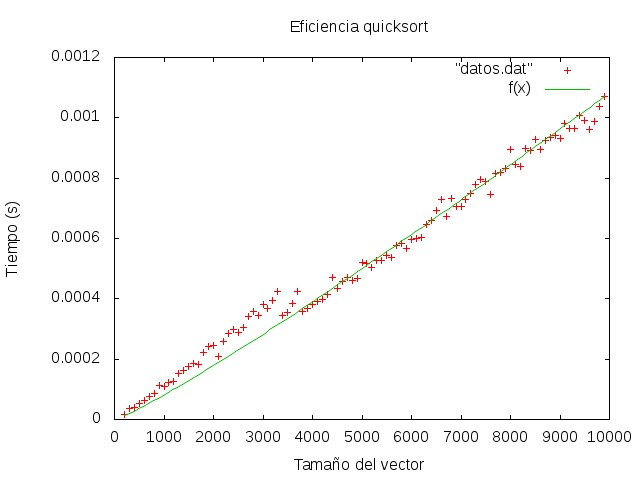
\includegraphics[scale=0.55]{../Graficas/Quicksort/quicksortO0_bruno.jpeg}					\end{center}	
	\end{alertblock}
\end{frame}

%%%%%%%%%%%%%%%%%%%%%%%%%%%%%%%%%%%%%%%%%%%%%%%%%%%%

\subsection{Comparación}
\begin{frame}{Algoritmos de ordenación}
	\begin{block}{Función}
	Se observa una diferencia notable entre los algoritmos $O(nlog_2(n))$ y los
	$O(n^2)$, casi no se aprecian los primeros.
	\end{block}
\end{frame}

\begin{frame}
	\begin{alertblock}{Imagen}
	\begin{center}
	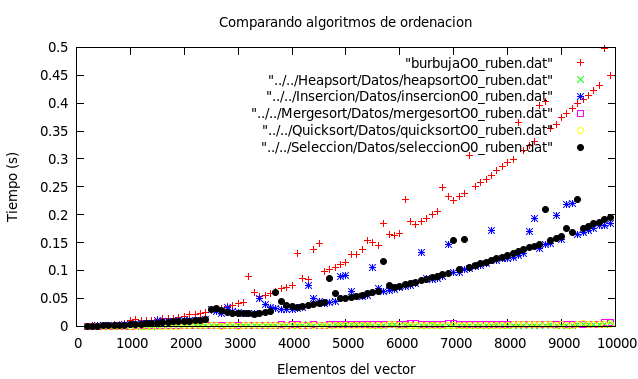
\includegraphics[scale=0.45]{../Graficas/todos.png}
	\end{center}
	\end{alertblock}
\end{frame}



% Resto de algoritmos
%%%%%%%%%%%%%%%%%%%%%%%%%%%%%%%%%%%%%%%%%%%%%%%%%%%%

\section{Resto de algoritmos}
\subsection{Fibonacci}
\begin{frame}{Fibonacci}
	\begin{block}{Función}
		Fibonacci
	\end{block}
	
	\begin{block}{Ajuste}
	$ f(x) = a\cdot   \left( \displaystyle\frac{1+\sqrt5}{2} \right)^x $

	{\ }
	$a               = 5.59738\cdot 10^{-9}      \pm 2.093\cdot 10^{-12}    (0.0374\%)$
	\end{block}
\end{frame}

\begin{frame}
	\begin{alertblock}{Imagen}
	\begin{center}
	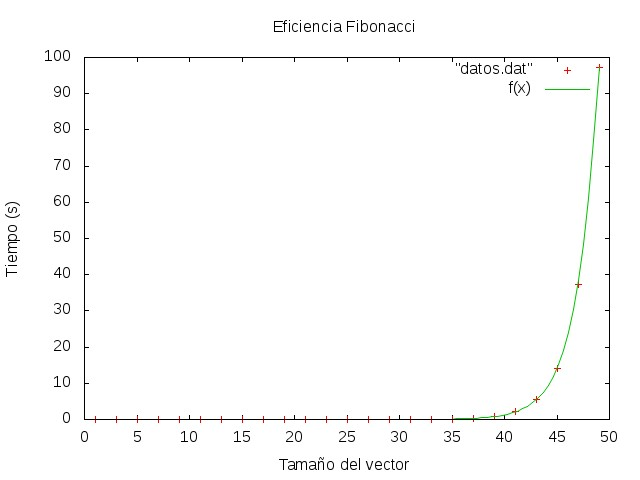
\includegraphics[scale=0.55]{../Graficas/Fibonacci/fibonacciO0_ruben.jpeg}
	\end{center}
	\end{alertblock}
\end{frame}


%%%%%%%%%%%%%%%%%%%%%%%%%%%%%%%%%%%%%%%%%%%%%%%%%%%%

\subsection{Hanoi}
\begin{frame}{Hanoi}
	\begin{block}{Función}
		Hanoi
	\end{block}
	
	\begin{block}{Ajuste}
	$f(x) = a\cdot(2^x) $
	
	$a               = 1.12636\cdot 10^{-8}      \pm 1.391\cdot 10^{-11}    (0.1235\%)$
	\end{block}
\end{frame}

\begin{frame}
	\begin{alertblock}{Imagen}
	\begin{center}
	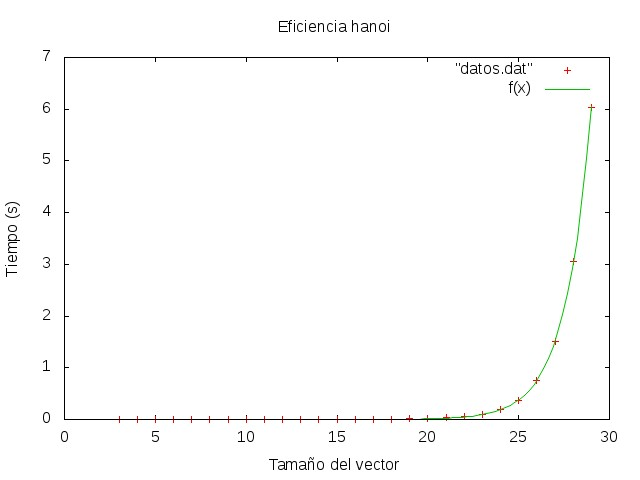
\includegraphics[scale=0.55]{../Graficas/Hanoi/hanoiO0_ruben.jpeg}
	\end{center}
	\end{alertblock}
\end{frame}


%%%%%%%%%%%%%%%%%%%%%%%%%%%%%%%%%%%%%%%%%%%%%%%%%%%%

\subsection{Floyd}
\begin{frame}{Floyd}
	\begin{block}{Función}
	Tipo de algoritmo con programación dinámica para encontrar el camino mínimo en grafos 		ponderados.
	\end{block}
	
	\begin{block}{Ajuste}
	$f(x) = a\cdot x^3 + b\cdot x^2 + c\cdot x + d $

	$\left\{ \begin{array}{c}
	a               = 1.11725\cdot 10^{-8}      \pm 3.725\cdot 10^{-10}    (3.334\%) \\
	b               = -2.27723\cdot 10^{-6}    \pm 6.692\cdot 10^{-7}    (29.39\%) \\
	c               = 0.00096037       \pm 0.0003713    (38.66\%) \\
	d               = -0.115743        \pm 0.06234      (53.86\%)
	\end{array}\right.$
	\end{block}
\end{frame}

\begin{frame}
	\begin{alertblock}{Imagen}
	\begin{center}
	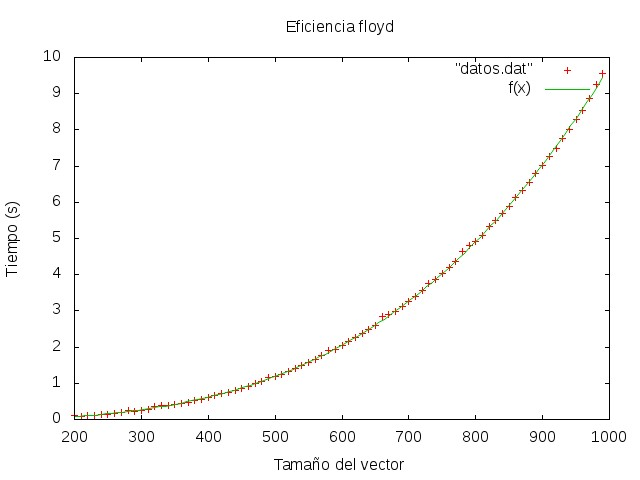
\includegraphics[scale=0.50]{../Graficas/Floyd/floydO0_ruben.jpeg}	
	\end{center}
	\end{alertblock}
\end{frame}


%%%%%%%%%%%%%%%%%%%%%%%%%%%%%%%%%%%%%%%%%%%%%%%%%%%%


\section{Optimización}
\subsection{Optimización}
\begin{frame}{Optimizando algoritmos}
	\begin{block}{Algoritmos}
	En este apartado optimizaremos diferentes algoritmos.
	\begin{itemize}
	\item Burbuja
	\item Quicksort
	\item Floyd
	\end{itemize}
	\end{block}
	
	\pause
	\begin{block}{Observación}
	Como podemos comprobar, por mucho que optimicemos el algoritmo de burbuja no llega a igualarse al mejor algoritmo de ordenación (en término medio), quicksort. La optimización más agresiva sin riesgo de pérdida de información es -O2 y llega a ser 10 veces más lento que quicksort sin optimización (con 10.000 elementos).
	\end{block}
\end{frame}


%%%%%%%%%%%%%%%%%%%%%%%%%%%%%%%%%%%%%%%%%


\begin{frame}{Burbuja optimizado}
	\begin{alertblock}{Imagen}
	\begin{center}
	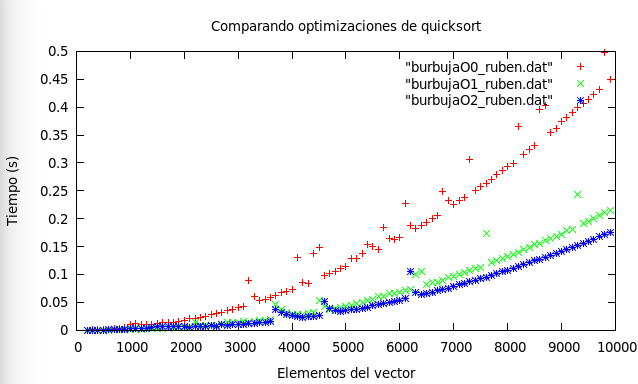
\includegraphics[scale=0.45]{../Graficas/Burbuja/burbuja_optimizacion.png}
	\end{center}
	\end{alertblock}
\end{frame}

\begin{frame}{Quicksort optimizado}
	\begin{alertblock}{Imagen}
	\begin{center}
	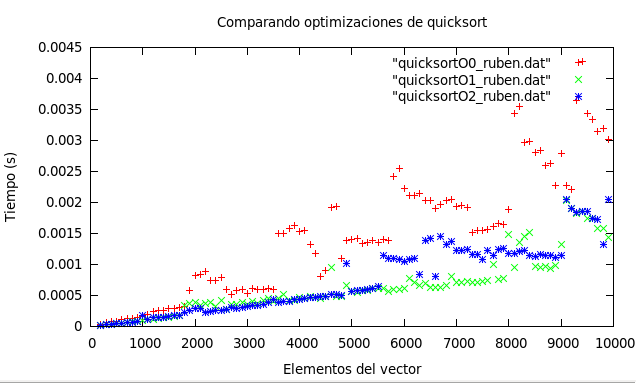
\includegraphics[scale=0.45]{../Graficas/Quicksort/quicksort_optimizacion.png}	
	\end{center}
	\end{alertblock}
\end{frame}


%%%%%%%%%%%%%%%%%%%%%%%%%%%%%%%%%%%%%%%%%%%%

\begin{frame}
	\begin{alertblock}{Conclusión}
	Esto es una prueba gráfica de que hay que tener en cuenta la eficiencia de los 				algoritmos, ya que la mejora hardware no es suficiente en caso de que tengamos 				restricciones de tiempo.
	\end{alertblock}
\end{frame}

\begin{frame}{Burbuja optimizado}
	\begin{alertblock}{Imagen}
	\begin{center}
	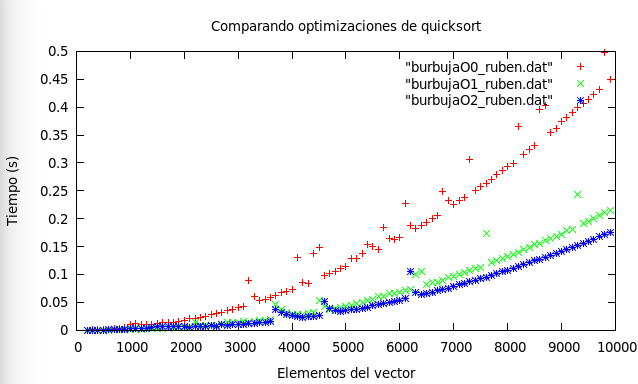
\includegraphics[scale=0.45]{../Graficas/Burbuja/burbuja_optimizacion.png}
	\end{center}
	\end{alertblock}
\end{frame}

%%%%%%%%%%%%%%%%%%%%%%%%%%%%%%%%%%%%%%%%%%%%%%%%%%%%
\begin{frame}{Floyd}
	\begin{block}{Algoritmo}
	El algoritmo floyd, tipo de algoritmo con programación dinámica para encontrar el 			camino mínimo en grafos ponderados.
	\end{block}
\end{frame}

\begin{frame}{Floyd}
	\begin{alertblock}{Imagen}
	\begin{center}
	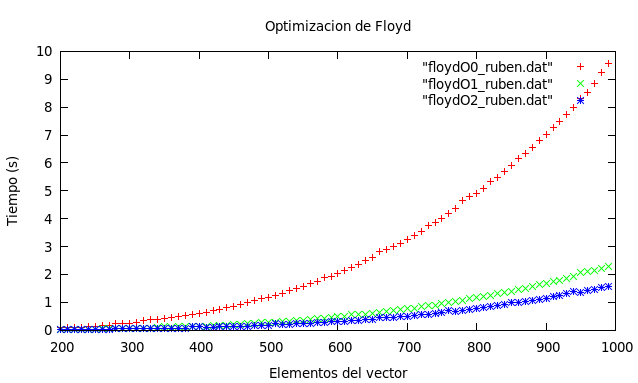
\includegraphics[scale=0.45]{../Graficas/Floyd/floyd_optimizacion.png}
	\end{center}
	\end{alertblock}
\end{frame}

%%%%%%%%%%%%%%%%%%%%%%%%%%%%%%%%%%%%%%%%%%%%%%%%%%%%%
\section{Diferentes ordenadores}
\begin{frame}{Diferentes ordenadores}
	\begin{alertblock}{Imagen}
	\begin{center}
	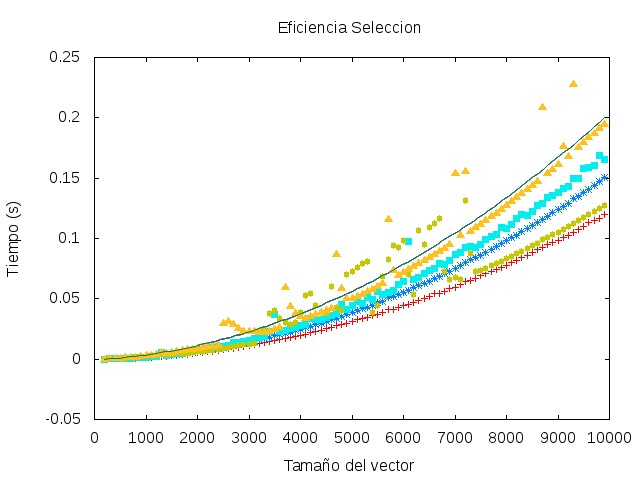
\includegraphics[scale=0.50]{../Graficas/Seleccion/total_Seleccion.jpeg}
	\end{center}
	\end{alertblock}
\end{frame}

%%%%%%%%%%%%%%%%%%%%%%%%%%%%%%%%%%%%%%%%%
\end{document}
